\documentclass[xcolor=dvipsnames]{beamer}
\usepackage{graphicx,epstopdf}
\usepackage{fancyhdr}
\usepackage{cite}
\usepackage{graphicx, epstopdf}
\usepackage{amsmath}
\usepackage{array}
\usepackage{epsfig}
\usepackage{amssymb}
\usepackage{subfigure}
\usepackage[ruled, lined,linesnumbered]{algorithm2e}
\usepackage{algorithmic}
\usepackage{tabularx}
\usepackage{rotating, boxedminipage}
\usepackage{rotating,multirow}
\usepackage{float}
\usepackage{algorithm2e}
\usetheme{Boadilla}
\usecolortheme[named=Blue]{structure}
\setbeamertemplate{items}[square]
\setbeamertemplate{caption}[numbered]
\setbeamertemplate{caption}[small]
\usepackage[absolute,overlay]{textpos}
\newenvironment{reference}[2]{%
  \begin{textblock*}{\textwidth}(#1,#2)
     \bgroup\fontsize{6pt}{\baselineskip}\selectfont\color[RGB]{0,112,192}}{\egroup\end{textblock*}}

\begin{document}
    \title[Evolutionary Multiobjective Optimization]{Sampling in Latent Space for a Multiobjective Estimation of Distribution Algorithm}
    \author{Bing Dong}
    \institute[East China Normal University]{East China Normal University, Shanghai, China}
    \logo{
\includegraphics[height=0.5cm,width=3.0cm]{university-logo-ecnu}\vspace{230pt}}
    \date{\today}
    \begin{frame}
        \titlepage
    \end{frame}
    \setbeamertemplate{section in toc}[square]
    \begin{frame}
        \frametitle{Outline}
        \tableofcontents
    \end{frame}

    \section{Background}
    \begin{frame}
    \frametitle{Definition}
    Multiobjective optimization problems (MOPs) can be defined as follows in this paper:
    \begin{equation}
    \begin{array}{rl}
    \mbox{min} & F(x) = (f_1(x), \cdots, f_m(x))\\
    \mbox{s.t} & x \in \Omega
    \end{array}
    \label{MOP}
    \end{equation}

    \begin{itemize}
    \item $x=(x_1, \cdots, x_n)^T\in R^n$ is a decision variable vector,
    \item $\Omega=\Pi_{i=1}^{n}[a_i, b_i] \subset R^n$ is the feasible region of the search space,
    \item $f_i: R^n \rightarrow R, i=1, \cdots, m$, is a continuous mapping,
    \item $F(x)$ is an objective vector.
    \end{itemize}
    \end{frame}
    
    \begin{frame}
    \frametitle{The algorithm framework of EDA}
    \begin{algorithm}[H]
    \label{alg2}
    \textbf{Initialization}: Initial the $Pop(t)$ randomly, and $t$ is the generation.
    
    \While{not terminate}
    {
    \textbf{Modelling}: Build a probabilistic model $p(x)$ according to the statistical information of the $Pop(t)$.
    
    \textbf{Sampling}: Generate a new solution set $Q$ by sampling from the built probabilistic model $p(x)$.
    
    \textbf{Selection}: Select from $Q\cup{Pop(t)}$ to construct the next population $Pop(t+1)$. The selection criterion is the objective function value.
    $t=t+1$
    }
    \end{algorithm}
    \end{frame}
    
    \begin{frame}
    \frametitle{RM-MEDA}
    Under mild smoothness conditions, the PS of a continuous MOP is a piecewise continuous $(m-1)$-dimensional manifold ($m$ is the number of objectives). This regularity property has been applied in the \emph{regularity model based multiobjective estimation of distribution algorithm (RM-MEDA)}
    \begin{figure}
    \centering
    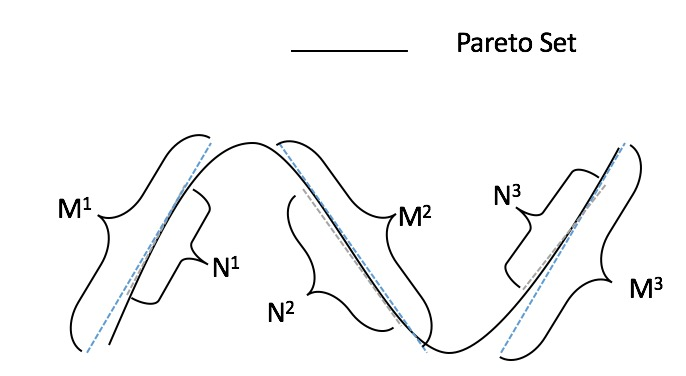
\includegraphics[width=0.5\columnwidth]{pareto.png}
    \caption{An illustration of model building and sampling in RM-MEDA.}
    \end{figure}
    \end{frame}

    \begin{frame}
    \frametitle{RM-MEDA}
    \begin{figure}
    \centering
    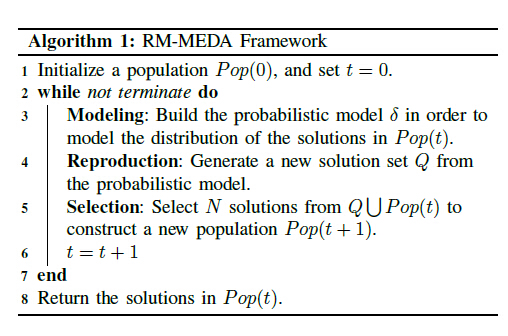
\includegraphics[width=0.5\columnwidth]{alg1.jpg}
    \caption{The framework of RM-MEDA}

    \end{figure}
    \begin{itemize}
    \item $t$ is the generation counter.
    \item $Pop(t)=\{x^1,x^2, \cdots x^N\}$ is the population at generation $t$.
    \item $\delta = \zeta + \varepsilon$ is the probabilistic model built in RM-MEDA.
    \item $Q$ is a new solution set sampled from the probabilistic model.
    \end{itemize}
    \end{frame}

    \begin{frame}
    \frametitle{Extension scale in RM-MEDA}
    \begin{figure}[htbp]
    \centering
    \subfigure[F1]{\includegraphics[ width=3.7cm, height=2.9cm]{figs/box_f1.eps}}
    \subfigure[F2]{\includegraphics[ width=3.7cm, height=2.9cm]{figs/box_f2.eps}}
    \subfigure[F3]{\includegraphics[ width=3.7cm, height=2.9cm]{figs/box_f3.eps}}
    \subfigure[F4]{\includegraphics[ width=3.7cm, height=2.9cm]{figs/box_f4.eps}}
    \subfigure[F5]{\includegraphics[ width=3.7cm, height=2.9cm]{figs/box_f5.eps}}
    \end{figure}
    \end{frame}

    \begin{frame}
    \frametitle{Extension scale in RM-MEDA}
    \begin{figure}[htbp]
    \centering
    \subfigure[F6]{\includegraphics[ width=3.7cm, height=2.9cm]{figs/box_f6.eps}}
    \subfigure[F7]{\includegraphics[ width=3.7cm, height=2.9cm]{figs/box_f7.eps}}
    \subfigure[F8]{\includegraphics[ width=3.7cm, height=2.9cm]{figs/box_f8.eps}}
    \subfigure[F9]{\includegraphics[ width=3.7cm, height=2.9cm]{figs/box_f9.eps}}
    \subfigure[F10]{\includegraphics[ width=3.7cm, height=2.9cm]{figs/box_f10.eps}}
    \end{figure}
    \end{frame}
    \section{DES}
    \begin{frame}
    \frametitle{mutation scheme}
    \begin{figure}
    \centering
    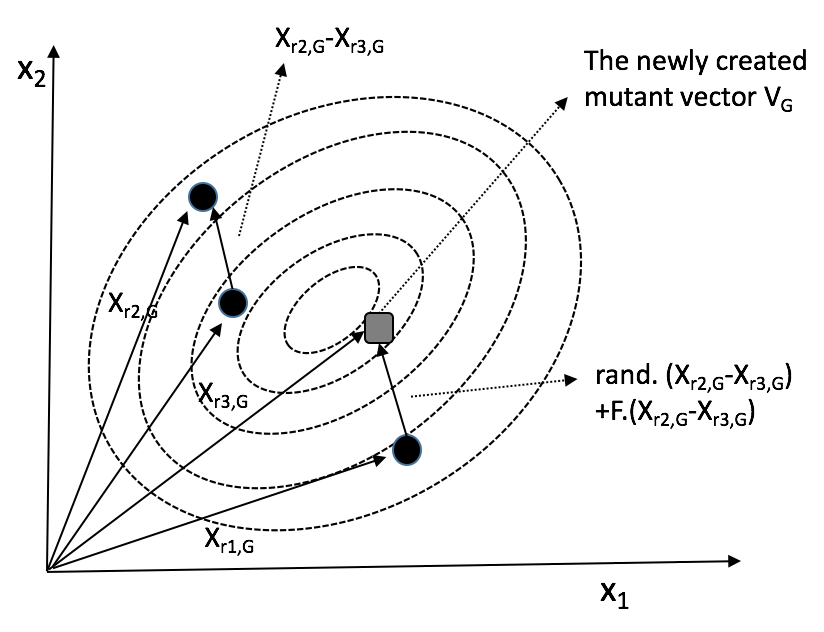
\includegraphics[width=0.3\columnwidth]{mutation1.png}
    \caption{The schema of the mutation}
    \end{figure}
    \begin{equation}
    \label{DE}
    X=X_{r_1}+rand\cdot(X_{r_2}-X_{r_3})+F\cdot(X_{r_2}-X_{r_3})
    \end{equation}

    \begin{itemize}
    \item $X_{r_1}$, $X_{r_2}$, $X_{r_3}$ are sampled randomly from the population
    \item $r_1$, $r_2$ and $r_3$ are mutually exclusive integers selected randomly from 1 to $NP$
    \item $F$ is the scaling factor
    \end{itemize}
    \end{frame}
    \begin{figure}
    \centering
    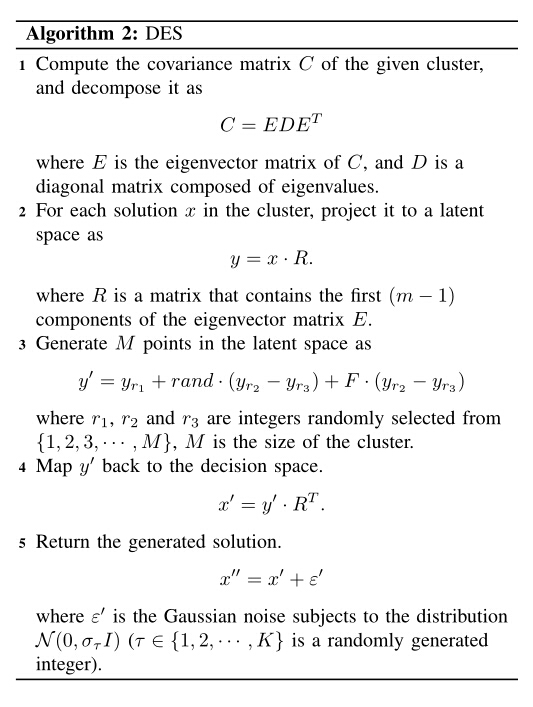
\includegraphics[width=0.5\columnwidth]{alg2.jpg}
    \caption{The framework of DES}
    \end{figure}

    \begin{frame}
    \begin{figure}
    \centering
    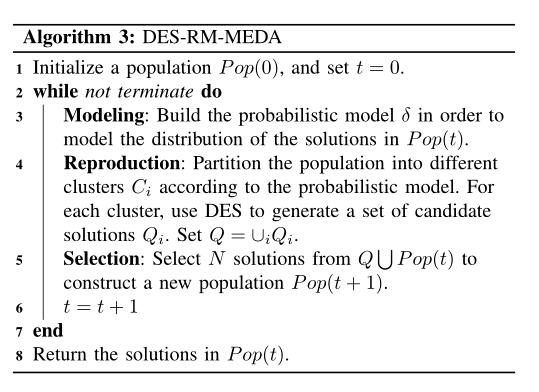
\includegraphics[width=0.5\columnwidth]{alg3.jpg}
    \caption{The framework of DES-RM-MEDA}
    \end{figure}
    \end{frame}
    \section{Experiment results}
    \begin{frame}
    \frametitle{Experimental settings}
    The 10 test instances, $F1-F10$, introduced in RM-MEDA are used as the benchmark problems.
    \begin{itemize}
    \item \emph{Initialization of the population}: The initial population in algorithms is randomly generated.
    \item \emph{The number of new trial solutions generated}: 100 for instances ($F3$, $F7$, $F9$), and 200 for other instances.
    \item \emph{The number of decision variables}: 30
    \item \emph{The number of clusters}: 5
    \item\emph{The scaling factor $F$}: 0.4
    \item\emph{The number of runs}: 30
    \item\emph{The number of generation}: 100 for instances ($F1$, $F2$, $F5$, $F6$), 200 for instances $F4$ and $F8$, and 1000 for instances $F3$, $F7$ and $F9$.
    \end{itemize}
    \end{frame}

    \begin{frame}
    \frametitle{The sensitivity of the F}
    \begin{figure}[htbp]
    \centering
    \subfigure[F1-F5]{\includegraphics[ width=4cm, height=3.2cm]{figs/f1_f5.eps}}
    \subfigure[F6-F9]{\includegraphics[ width=4cm, height=3.2cm]{figs/f6_f9.eps}}
    \subfigure[F10]{\includegraphics[ width=4cm, height=3.2cm]{figs/f10.eps}}
    \end{figure}
    \end{frame}

    \begin{frame}
    \frametitle{Wilcoxon's rank sum test}
    \begin{figure}
    \centering
    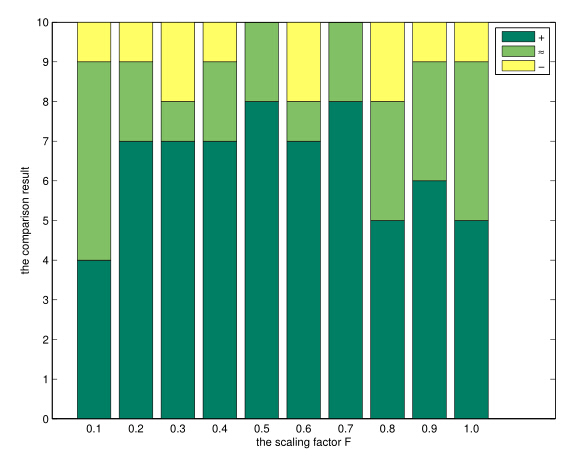
\includegraphics[width=0.6\columnwidth]{f_performance.jpg}
    \caption{The compariosn of RM-MEAD and RM-MEDA-DES with different settings of F}
    \end{figure}
    \end{frame}

    \begin{frame}
    \frametitle{Comparison study}
    \begin{figure}[htbp]
    \centering
    \subfigure[F1]{\includegraphics[ width=3.7cm, height=2.8cm]{figs/f1_igd.eps}}
    \subfigure[F2]{\includegraphics[ width=3.7cm, height=2.8cm]{figs/f2_igd.eps}}
    \subfigure[F3]{\includegraphics[ width=3.7cm, height=2.8cm]{figs/f3_igd.eps}}
    \subfigure[F4]{\includegraphics[ width=3.7cm, height=2.8cm]{figs/f4_igd.eps}}
    \subfigure[F5]{\includegraphics[ width=3.7cm, height=2.8cm]{figs/f5_igd.eps}}
    \caption{The dashed line is RM-MEDA, and the solid line is RM-MEDA-DES}
    \end{figure}    
    \end{frame}

    \begin{frame}
    \frametitle{Comparison study}
    \begin{figure}[htbp]
    \centering
    \subfigure[F6]{\includegraphics[ width=3.7cm, height=2.8cm]{figs/f6_igd.eps}}
    \subfigure[F7]{\includegraphics[ width=3.7cm, height=2.8cm]{figs/f7_igd.eps}}
    \subfigure[F8]{\includegraphics[ width=3.7cm, height=2.8cm]{figs/f8_igd.eps}}
    \subfigure[F9]{\includegraphics[ width=3.7cm, height=2.8cm]{figs/f9_igd.eps}}
    \subfigure[F10]{\includegraphics[ width=3.7cm, height=2.8cm]{figs/f10_igd.eps}}
    \caption[small]{The dashed line is RM-MEDA, and the solid line is RM-MEDA-DES}
    \end{figure}   
    \end{frame}

    \begin{frame}
    \frametitle{Comparison study}
    \begin{figure}
    \centering
    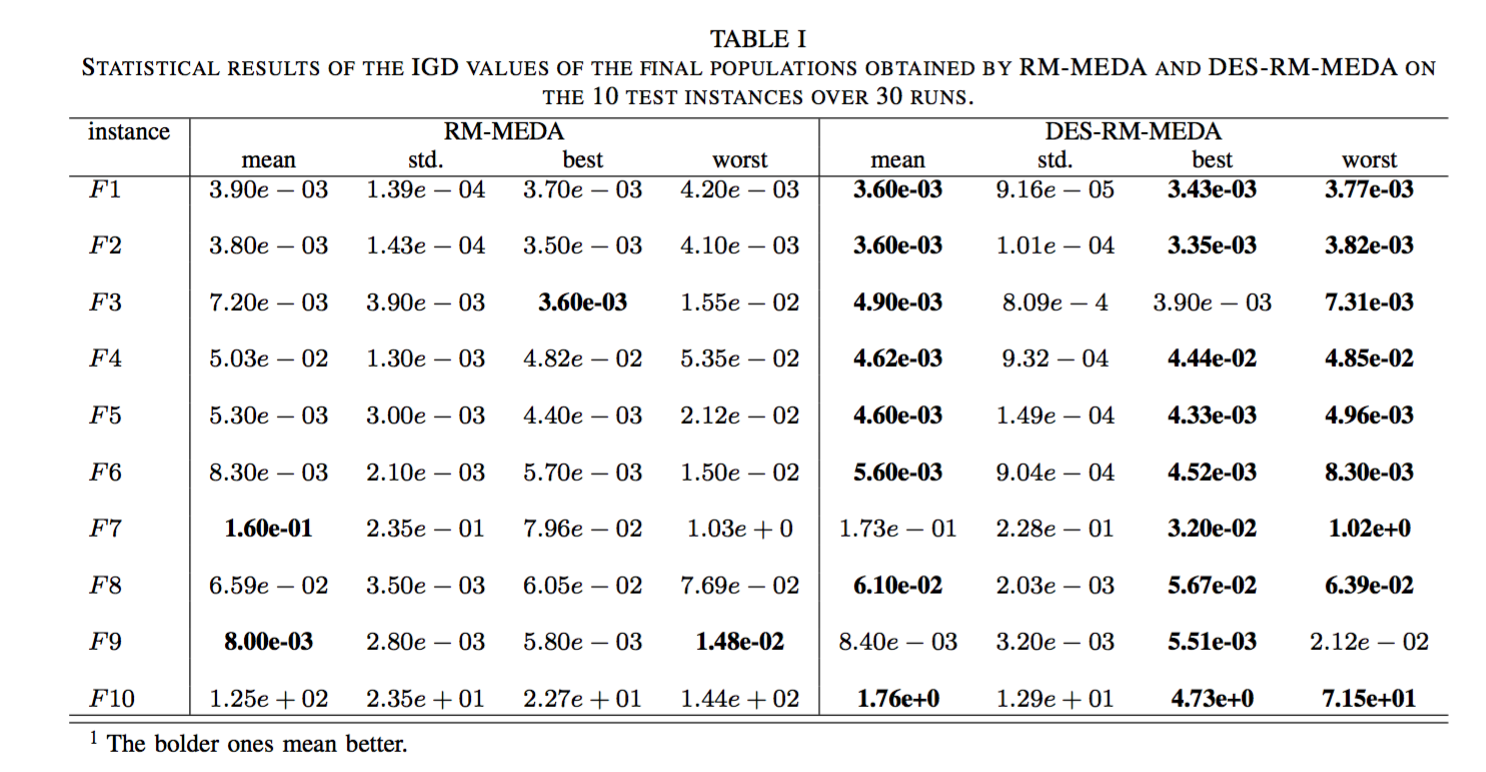
\includegraphics[width=1\columnwidth]{tab1.png}
    \end{figure}
    \end{frame}
    \section{Conclusions}
        \begin{frame}
        \frametitle{Conclusions}
        \textbf{Main contributions}
        \begin{itemize}
        \item A new sampling strategy for multiobjective estimation of distribution algorithm.
        \item Addressing to the issue of the extension scale setting in RM-MEDA.
        \end{itemize}
        This paper proposed a DES scheme to generate points in the latent space. The basic idea is to project the parent solutions
        into the latent space, and use a DE mutation operator to generate new points in the latent space based on the projected points, and finally map the points back to
        to the decision space added with Gaussian noise to generate offspring solutions. The DES is implemented into RM-MEDA to improve the performance. The results are impressive.
        \end{frame}

        \begin{frame}
        \frametitle{The future work}
       	\begin{itemize}
       	\item To exploit the deeper application of the DES. There is the possibility to apply the DES to other MOEAs.
       	\item It is valuable to explore the hybrid menthod of the DE and EDA. Though DE/EDA has been proposed, it is still interesting to explore the potential of this method.
       	And the arrange of the resources of DE and EDA is also an interesting topic.
       	\end{itemize}
       \end{frame}
    \section*{thx}
        \begin{frame}
        \begin{center}
        %\structure
        \fontsize{60pt}{\baselineskip}\selectfont \structure{Thanks!}
        \end{center}
        \begin{reference}{0mm}{80mm}
        \begin{itemize}
        \item  B. Dong, A. Zhou, and G. Zhang, Sampling in Latent Space for a Multiobjective Estimation of Distribution Algorithm, 2016 IEEE Congress on Evolutionary Computation (CEC), 2016.       
        \end{itemize}
        \end{reference}
        \end{frame}
\end{document}
